\documentclass[a4paper,10pt]{article}
\usepackage{polski}
\usepackage[utf8]{inputenc}
\usepackage{graphicx}
\usepackage{listings}
\usepackage{xcolor}
\usepackage{tabularx}
\usepackage{adjustbox}
\usepackage{amssymb}
\usepackage{amsmath}
\usepackage{float}

%opening
\author{Tomasz Zakrzewski, tz336079}
\title{Praca domowa z RPiS}

% Margins
\topmargin=-0.45in
\evensidemargin=0in
\oddsidemargin=0in
\textwidth=6.5in
\textheight=9.0in
\headsep=0.25in

\begin{document}

\maketitle

\section{Wstęp}
Praca domowa miała na celu ustalenie lepszego estymatora następujągego eksperymentu:

W bibliotece jest pewna ilość książek ($a$). Wybieramy losowo pewne $k$ książek i patrzymy na ich numery 
(wszystkie książki w bibliotece ponumerowane są od 1 do $a$). Ile jest książek w całej bibliotece?

Rozważane estymatory to:
\begin{itemize}
 \item ``mean'': średnia wszystkich pomiarów,
 \item ``max'': $max \frac{n + 1}{n}$, gdzie $max$ to maksymalny z poznanych $n$ elementów. 
\end{itemize}

\section{Eksperyment}
Statystyczne eksperymenty w celu wykazania wyższości jednego z dwóch proponowanych estymatorów zostały wykonane za pomocą programu R.
Napisany skrypt przeprowadzał 2 pomiary:
\begin{enumerate}
 \item W pierwszym eksperymencie, dla ustalonych k i a (wybranych arbitralnie) przeprowadzanych była pewna ilość (1000) prób. Próba polegała na 
 wylosowaniu $k$ próbek z rozkładu normalnego z przedziału $[1; a]$
 \item W drugim eksperymencie pierwszy był przeprowadzany dla coraz większych wartości $k$ i liczone było standardowe odchylenie wyniku. Wartość
 $a$ wynosiła $100$.
\end{enumerate}

\section{Wyniki}
Najlepszym przybliżeniem okazało się ``max''.
Na poniższych wykresach próby typy 1., metoda ``max'' oznaczona jest kolorem niebieskim, a ``mean'' czerwonym. Ostatni wykres przedstawia
eksperyment 2.

\begin{figure}[h!]
       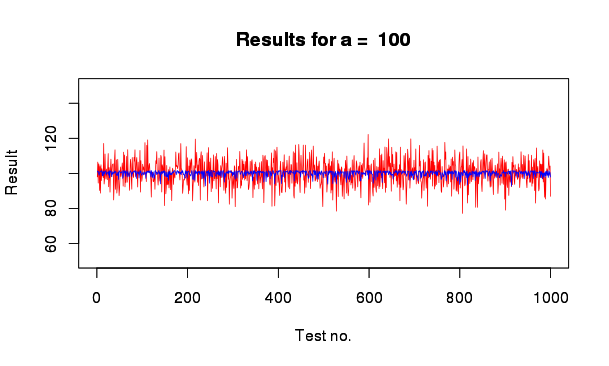
\includegraphics[width=0.5\textwidth]{result100.png}
       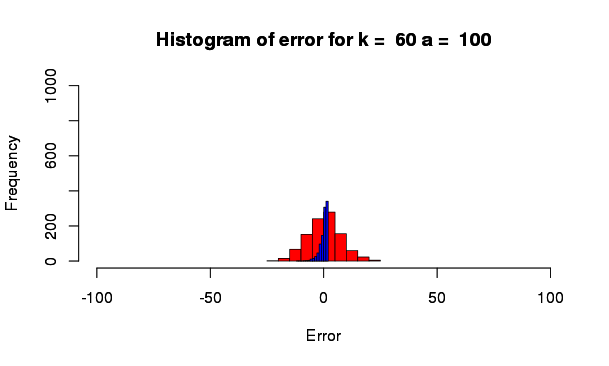
\includegraphics[width=0.5\textwidth]{errorHistogram100.png}
\end{figure}

\begin{figure}[h!]
       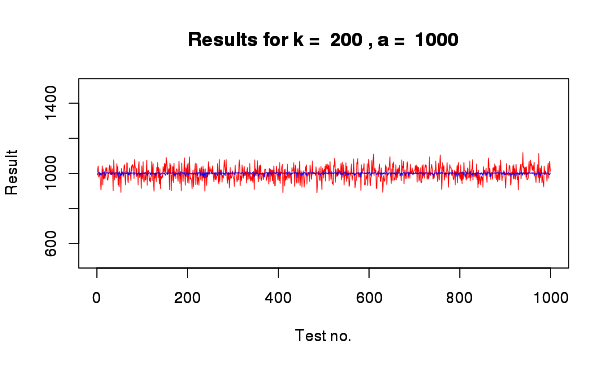
\includegraphics[width=0.5\textwidth]{result1000.png}
       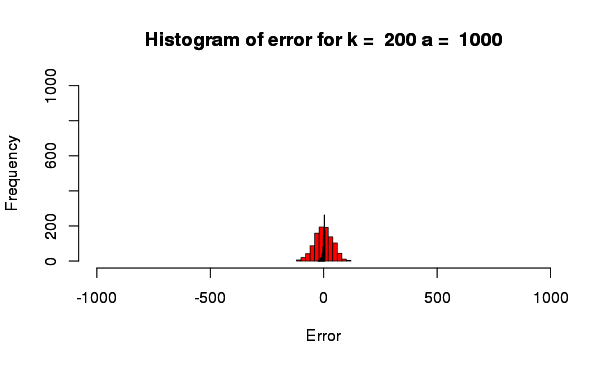
\includegraphics[width=0.5\textwidth]{errorHistogram1000.png}
\end{figure}

\begin{figure}[h!]
       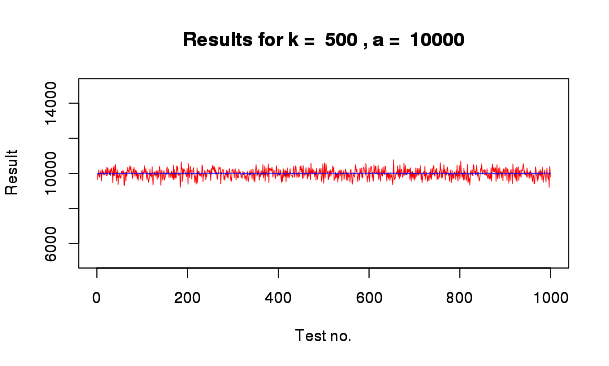
\includegraphics[width=0.5\textwidth]{result10000.png}
       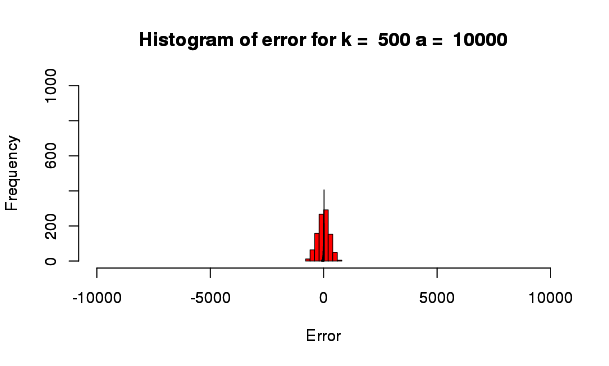
\includegraphics[width=0.5\textwidth]{errorHistogram10000.png}
\end{figure}

\begin{figure}[h!]
       \centering
       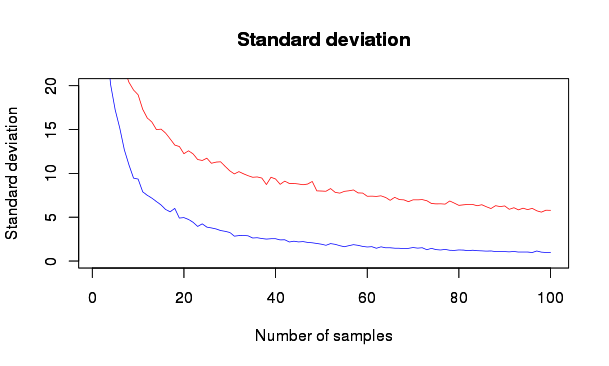
\includegraphics[width=0.5\textwidth]{stddev.png}
\end{figure}

\section{Uzasadnienie}
Na wykresach pierwszego eksperymentu widać wyraźnie, że wartości uzyskiwane metodą ``max'' oscylują bardzo blisko faktycznego wyniku, podczas gdy 
``mean'' ma średnio większy błąd. Ponadto, odchylenie standardowe w eksperymencie 2. maleje bardzo szybko dla ``max'' i już dla ilości próbek
stanowiących ok. $20\%$ całkowitej ilości badanych obiektów, jest mniejsze niż $5$.

\section{Uwagi}
Ciekawą obserwacją jest, że ze względu na wzór metody ``max'', wyniki uzyskiwane nią bardzo rzadko przekraczają szukaną wartość i można dosyć 
bezpiecznie przyjąć, że metoda ta osiąga prawie zawsze wartości mniejsze lub równe oczekiwanemu wynikowi, podczas gdy ``mean'' może wyraźnie
zawyżać wynik.

\end{document}